\documentclass[UTF8,aspectratio=169]{ctexbeamer}
\usetheme{Madrid}
\usecolortheme{default}
\usepackage{amsmath}
\usepackage{booktabs}
\usepackage{array}
\usepackage{xcolor}
\usepackage{xurl}
\usepackage{colortbl}
\usepackage{graphicx}

\newcommand{\good}[1]{\textcolor{green!45!black}{#1}}
\newcommand{\warn}[1]{\textcolor{red!65!black}{#1}}
\newcommand{\bluenote}[1]{\textcolor{blue!65!black}{#1}}
\newcolumntype{L}[1]{>{\raggedright\arraybackslash}p{#1}}
\definecolor{winrow}{RGB}{220,240,220}
\definecolor{softrow}{RGB}{232,242,255}
\definecolor{warnrow}{RGB}{250,228,228}

\AtBeginSection[]{%
  \begin{frame}{路线图}
    \footnotesize
    \tableofcontents[currentsection, hideallsubsections]
  \end{frame}}

\title[残差族头]{残差族头：让已部署喷雾穿透代理模型可扩展}
\subtitle{冻结骨干上的加性残差，以及低成本族适配器的边界}
\author{Mie Spray Postprocessing Project}
\date{2026-06-01}

\begin{document}

\begin{frame}
  \titlepage
\end{frame}

% ------------------------------------------------------------------
\begin{frame}{这组 slides 的主线}
\small
第5章已经得到一个可用于筛选的 Stage-3 代理模型。这里追问一个部署问题：
\begin{center}
\emph{能不能让模型自然支持新的喷嘴族，同时不牺牲已经得到的精度？}
\end{center}

\vspace{0.35em}
\textbf{所有实验共享同一个原则：}
\[
  \boxed{\ \text{prediction}=\underbrace{\text{shared backbone}}_{\text{冻结、热启动}}
  +\underbrace{\text{small per-family residual}}_{\text{训练、零初始化}}\ }
\]

\vspace{0.35em}
\begin{enumerate}\setlength\itemsep{2pt}
  \item 第5章留下的两个缺口：部署可扩展性与精度上限。
  \item 冻结骨干上的加性残差：为什么它是结构性 fallback。
  \item 域内性能爬升：residual head $\to$ FiLM $\to$ multi-task SVGP。
  \item 鲁棒性：LONO 迁移与 lv2/lv3 数据敏感性。
  \item 边界：低成本 adapter 在哪里失效。
  \item 对论文叙事的补充：哪些结论被加强，哪些仍要保守。
\end{enumerate}
\end{frame}

% ==================================================================
\section{第5章留下的起点}

% ------------------------------------------------------------------
\begin{frame}{论文主模型的当前位置}
\small
第5章报告了三阶段 MLP 筛选代理模型，以及一个 SVGP 替代骨干。这里仍使用同一张
\textbf{保守 uncensored CDF 点表}（542{,}565 个点），因此可以直接和 thesis 结果对齐。

\vspace{0.3em}
\begin{center}
\renewcommand{\arraystretch}{1.15}
\setlength{\tabcolsep}{5.5pt}
\begin{tabular}{@{}lrr@{}}
\toprule
\textbf{模型（uncensored CDF，542k 点）} & \textbf{RMSE [mm]} & \textbf{P50 RMSE [mm]} \\
\midrule
Hiroyasu--Arai 校准物理基线 & 10.261 & -- \\
Naber--Siebers + delay 物理基线 & 9.286 & -- \\
三阶段 MLP，5-seed 选定模型 & 4.265 & 2.848 \\
\rowcolor{softrow}
Stage-3 SVGP（论文最强点预测器） & \textbf{4.193} & \textbf{2.649} \\
\bottomrule
\end{tabular}
\end{center}

\vspace{0.35em}
\footnotesize
第5章的结论不是“MLP 全面胜出”：SVGP 在点预测和 LONO 迁移上更强；MLP 的优势是
域内保守覆盖、可审计工作流，以及 injection-onset 辅助头。LONO 中 Nozzle0 仍是跨设计族失败。
\end{frame}

% ------------------------------------------------------------------
\begin{frame}{两个尚未闭合的问题}
\small
\begin{columns}[T]
\column{0.5\textwidth}
\begin{block}{1. 部署 / 可扩展性}
已部署模型显式依赖喷嘴族。新增一个族时，要么硬编码 fallback，要么重新训练一个 head。
这不是一个干净的结构性答案。
\end{block}

\column{0.5\textwidth}
\begin{block}{2. 精度上限}
同一主表上，论文里最强的单模型是 SVGP（RMSE 4.193 mm）。能否沿用同一套
censoring-aware protocol，把精度继续推低？
\end{block}
\end{columns}

\vspace{0.55em}
\textbf{本研究的主张。} 把 family-aware Stage-3 模型改成
\emph{残差族头}：
\[
  \mu(x,f)=\mu_{\rm shared}(h(x))+\Delta_f(h(x))
\]
可以同时处理两个问题：新族有自然 fallback；在 SVGP 骨干上还能刷新主表精度。
\end{frame}

% ==================================================================
\section{理论：冻结骨干上的加性残差}

% ------------------------------------------------------------------
\begin{frame}{喷嘴族条件化的三种设计}
\small
设 $h(x)$ 是低维工况输入的共享表示（时间、幅值缩放、压力残差等）。喷嘴族 $f$ 可以用三种方式进入均值函数：

\vspace{0.2em}
\begin{center}
\renewcommand{\arraystretch}{1.22}
\setlength{\tabcolsep}{3.8pt}
\begin{tabular}{@{}L{3.0cm}L{4.4cm}L{2.8cm}r@{}}
\toprule
\textbf{设计} & \textbf{族信息如何进入} & \textbf{新族处理} & \textbf{CDF RMSE} \\
\midrule
one-hot 输入 & $f$ 作为特征进入共享 head $\mu(h,f)$ & 隐式外推 & 4.265 \\
\rowcolor{warnrow}
per-family head & 每个族一个 decoder $\mu_f(h)$ & \warn{需要 fallback / 新 head} & 5.056 \\
\rowcolor{winrow}
残差族头 & 共享均值 $+$ 小残差 $\mu_{\rm shared}+\Delta_f$ & \good{零残差 $\to$ 共享模型} & 4.631 \\
\bottomrule
\end{tabular}
\end{center}

\vspace{0.15em}
\begin{itemize}\setlength\itemsep{1pt}
  \item per-family head 有容量，但会碎片化数据：RMSE 从 single-head 的 4.265 升到 5.056。
  \item residual head 恢复大部分损失（5.056$\to$4.631），同时把新族 fallback 变成模型结构。
\end{itemize}
\end{frame}

% ------------------------------------------------------------------
\begin{frame}{残差族头：恒等热启动 + 结构性 fallback}
\small
\begin{columns}[T]
\column{0.55\textwidth}
\[
  \mu(x,f)=\mu_{\rm shared}(h(x))+\Delta_f(h(x)),\qquad
  \Delta_f\equiv0\ \text{at init}
\]
\textbf{残差学习视角。} 每个喷嘴族只学对强共享预测器的修正，而不是重新学习整张映射。
零初始化保证 step 0 等于已部署模型。

\vspace{0.25em}
\textbf{结构性 fallback。} 未见过的新族令 $\Delta_f\equiv0$，自然退回
$\mu_{\rm shared}$，不需要手写 \texttt{fallback\_family\_id}。

\vspace{0.25em}
\textbf{收缩先验。} \texttt{delta\_L2} 把族残差拉回共享模型，本质上是层级收缩：
在每族拟合和共享稳定性之间做权衡。

\column{0.45\textwidth}
\footnotesize
\begin{block}{参数高效迁移}
冻结 backbone，只训练很小的族模块：
\begin{itemize}\setlength\itemsep{1pt}
  \item trunk frozen: 334{,}720 params
  \item shared mean frozen: 16{,}641 params
  \item \good{trainable: 49{,}923}（$\Delta$ heads + log-var）
\end{itemize}
新增族就是新增 adapter，而不是重训整网。
\end{block}

\begin{block}{热启动映射}
\scriptsize
copy \texttt{trunk.*}; copy \texttt{log\_var\_head.*};
\texttt{mu\_heads.1}$\to$\texttt{mu\_shared\_head};
\texttt{delta\_heads.*} 零初始化，然后 10 epoch KD mimic。
\end{block}
\end{columns}
\end{frame}

% ------------------------------------------------------------------
\begin{frame}{同一原则的两个更强版本}
\small
\begin{block}{FiLM：不只调输出偏移，也调中间表示}
\[
  h_l'=\gamma_{f,l}\odot h_l+\beta_{f,l},\qquad
  \mu(x,f)=\mu_{\rm shared}(h_L')+\Delta_f(h_L')
\]
FiLM 在 trunk 内插入每族 affine modulation。恒等初始化
（$\gamma=1,\beta=0,\Delta_f=0$）保证热启动不被破坏。
\end{block}

\begin{block}{加性残差 multi-task SVGP：把同一想法搬到 GP 骨干}
\[
  g(x,f)=g_{\rm shared}(x)+\delta_f(x)
\]
共享 sparse variational GP 从 Stage-3 SVGP 热启动，每个喷嘴族再有一个残差 GP。
family id 只负责路由 residual，不进入 kernel 特征。未见族退回共享 GP。
这是一个 shared-plus-per-family 的加性层级 multi-task GP。
\end{block}

\vspace{0.2em}
\footnotesize
共同实验契约：\textbf{从部署 checkpoint 热启动，冻结骨干，只训练零/恒等初始化的每族残差。}
\end{frame}

% ------------------------------------------------------------------
\begin{frame}{结构图：Family Head vs Residual vs FiLM}
\small
\begin{center}
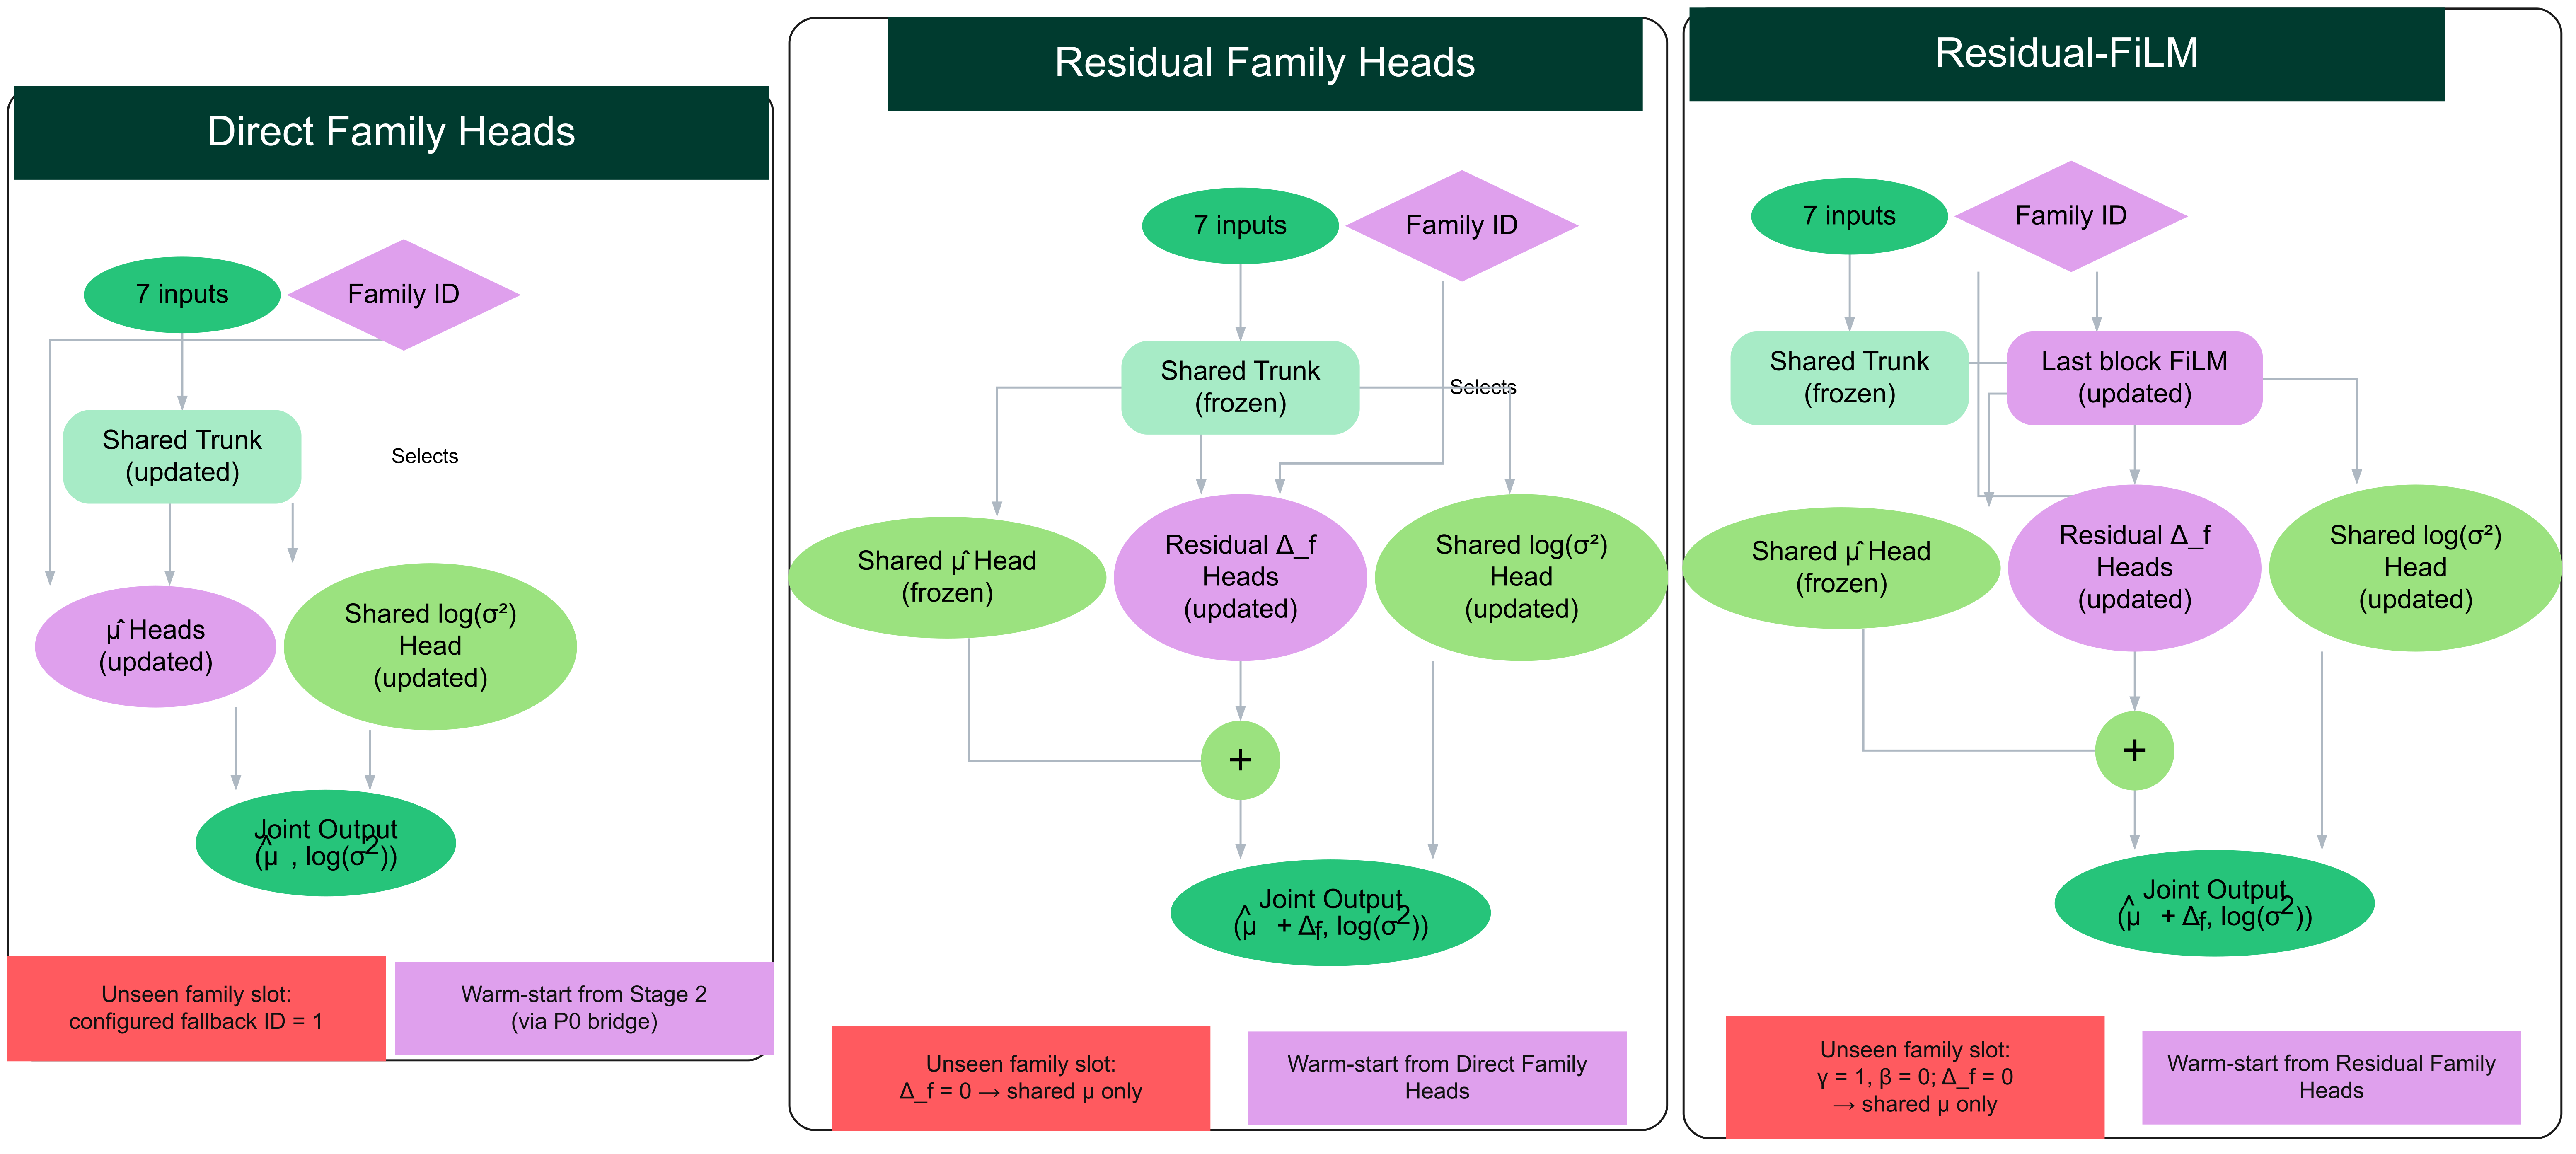
\includegraphics[width=0.96\textwidth,height=0.74\textheight,keepaspectratio]{figs/mlp_family_conditioning_architecture_simple.png}
\end{center}
\vspace{-0.2em}
\footnotesize
\centering
Direct head、残差、FiLM；cell 标出状态和 fallback。
\end{frame}

% ------------------------------------------------------------------
\begin{frame}{实验契约}
\small
\begin{block}{固定的 production baseline}
\begin{itemize}\setlength\itemsep{2pt}
  \item baseline run:
        \texttt{distill\_cdf\_family\_head\_v3\_FROZEN\_anchor\_off\_20260529\_213346}
        （部署版 per-family-head，CDF RMSE 5.056）。
  \item feature contract: \texttt{a\_dp050\_plus\_pressures}; device CUDA。
  \item evaluation: canonical point tables
        \texttt{cdf\_uncensored}, \texttt{p50\_observed}, \texttt{q1\_grid\_all}。
\end{itemize}
\end{block}

\vspace{0.25em}
\begin{center}
\renewcommand{\arraystretch}{1.15}
\begin{tabular}{@{}L{4.0cm}L{8.4cm}@{}}
\toprule
\textbf{实验轴} & \textbf{取值 / 设定} \\
\midrule
Residual shrinkage & \texttt{0}, \texttt{1e-4}, \texttt{1e-3}, \texttt{1e-2} \\
Mimic warm-up & 10 epochs；teacher 为部署 production model \\
Refinement & 150 max epochs, patience 20, trunk frozen \\
Trainable params & 49{,}923：residual deltas + shared log-var head \\
\bottomrule
\end{tabular}
\end{center}
\end{frame}

% ==================================================================
\section{域内性能爬升}

% ------------------------------------------------------------------
% 压缩后的训练/结果总览：一页三图 + 一句结论。
\begin{frame}{系统性族差异 $\Rightarrow$ 残差微调有用}
\small
\begin{columns}[T,onlytextwidth]
\column{0.34\textwidth}
\centering

\includegraphics[width=\linewidth,height=0.52\textheight,keepaspectratio]{figs/injector_scatter_all_nozzles.png}\\[0.3em]
{\scriptsize \textbf{数据} —— 全部喷嘴的无量纲贯穿距离散点：各喷嘴族\emph{系统性地}分层，并非噪声。}
\column{0.34\textwidth}
\centering
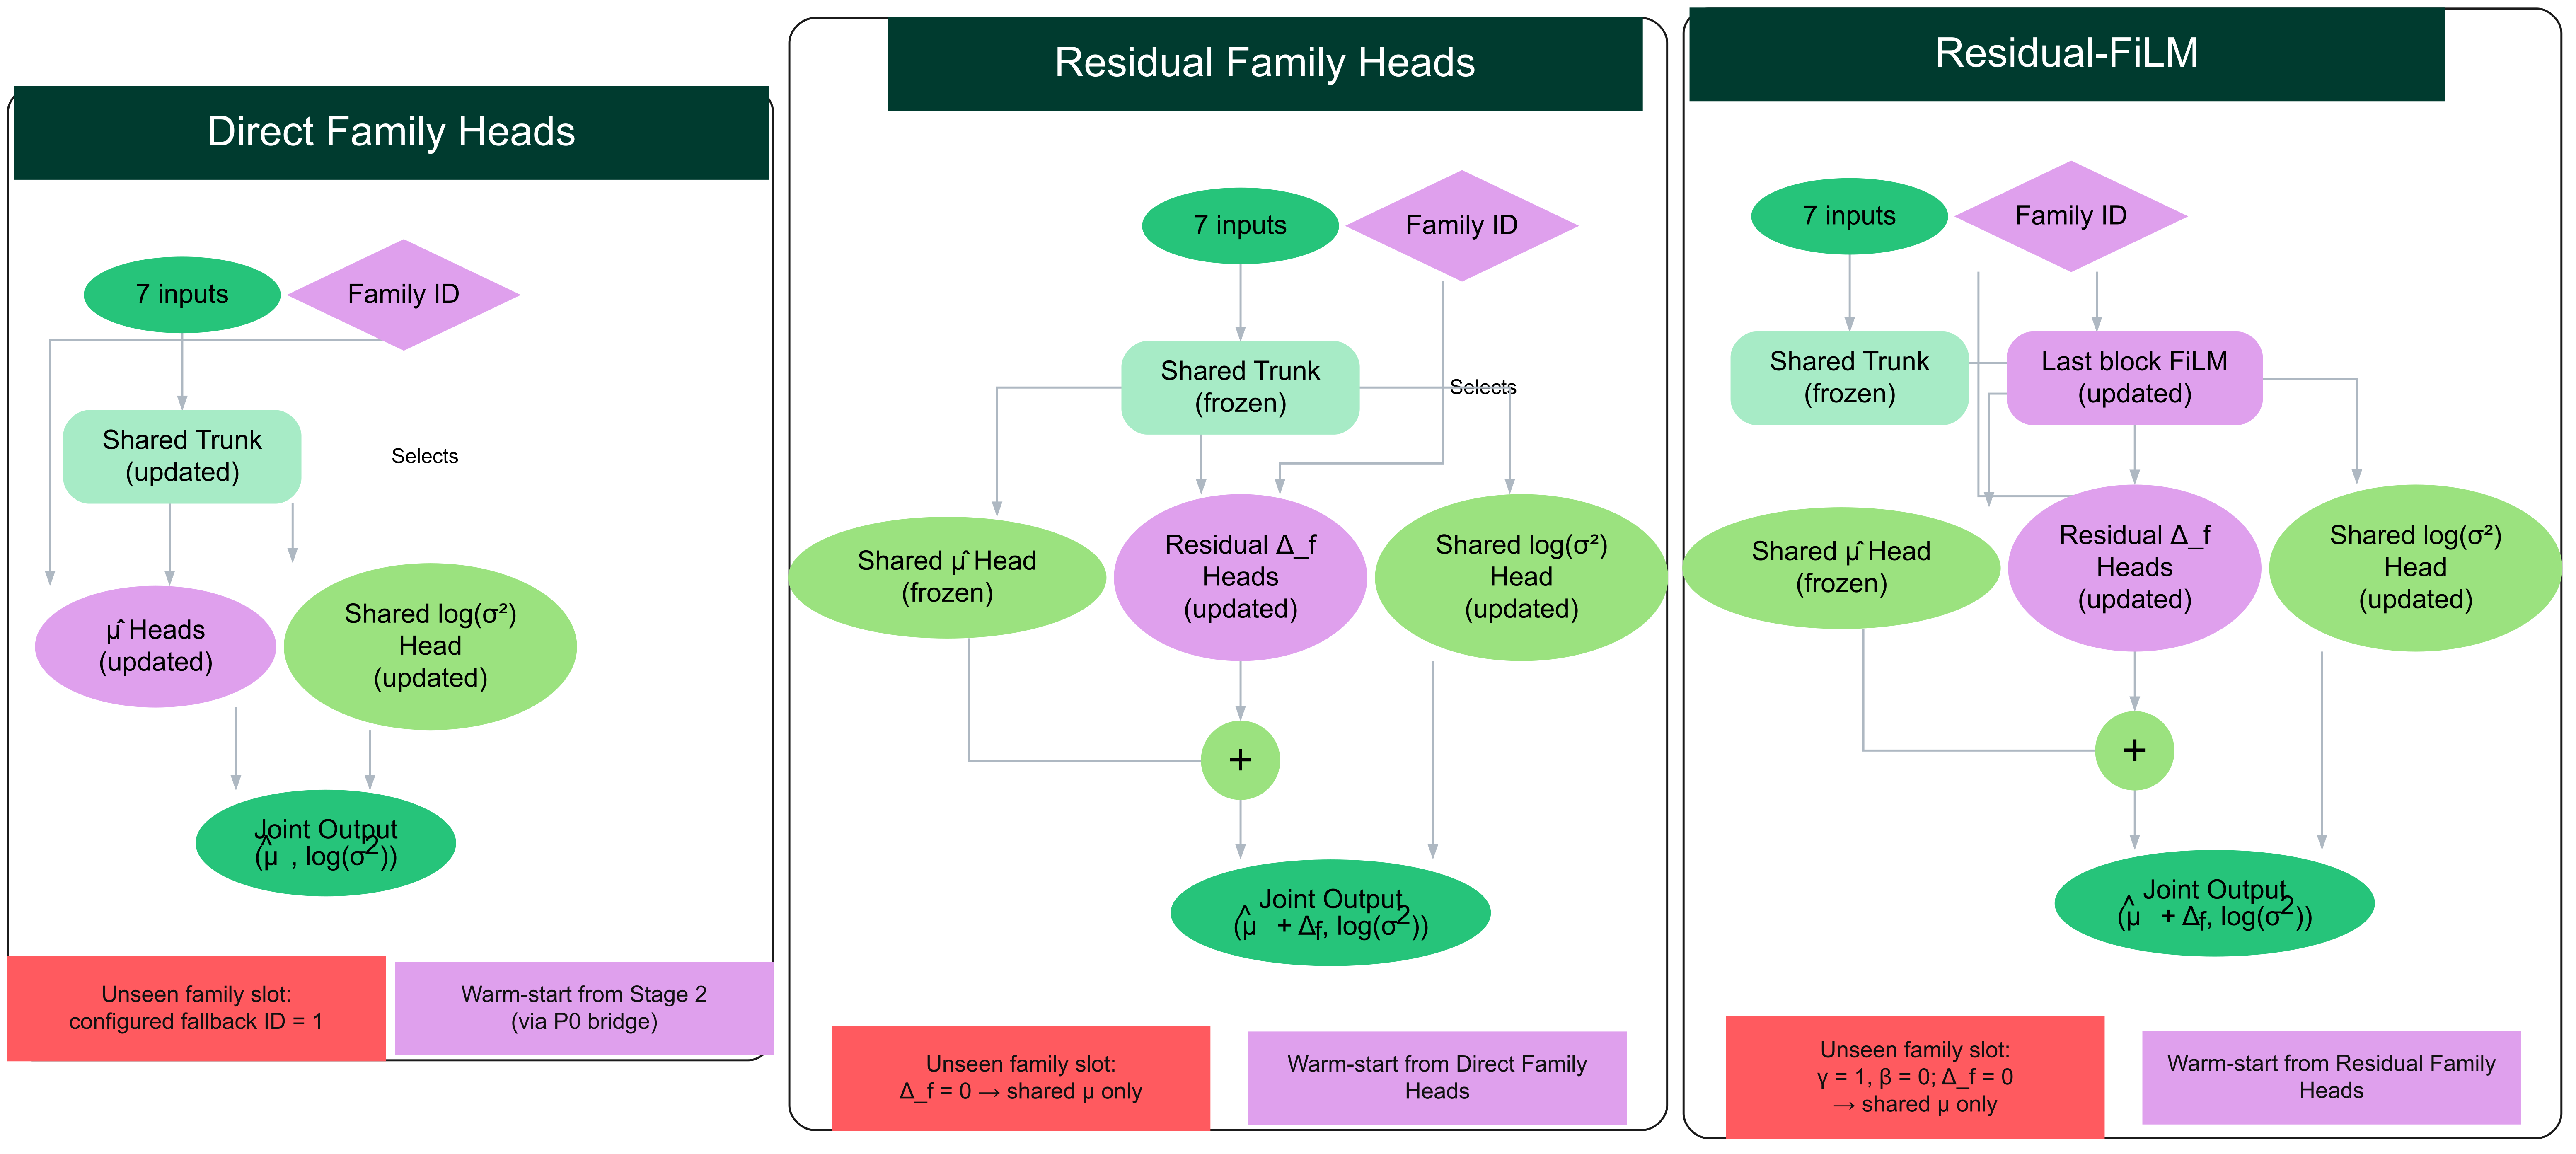
\includegraphics[width=\linewidth,height=0.52\textheight,keepaspectratio]{figs/mlp_family_conditioning_architecture_simple.png}\\[0.3em]
{\scriptsize \textbf{架构} —— direct family head、加性残差和最后一层 FiLM；未知族使用显式 fallback。}
\column{0.32\textwidth}
\centering
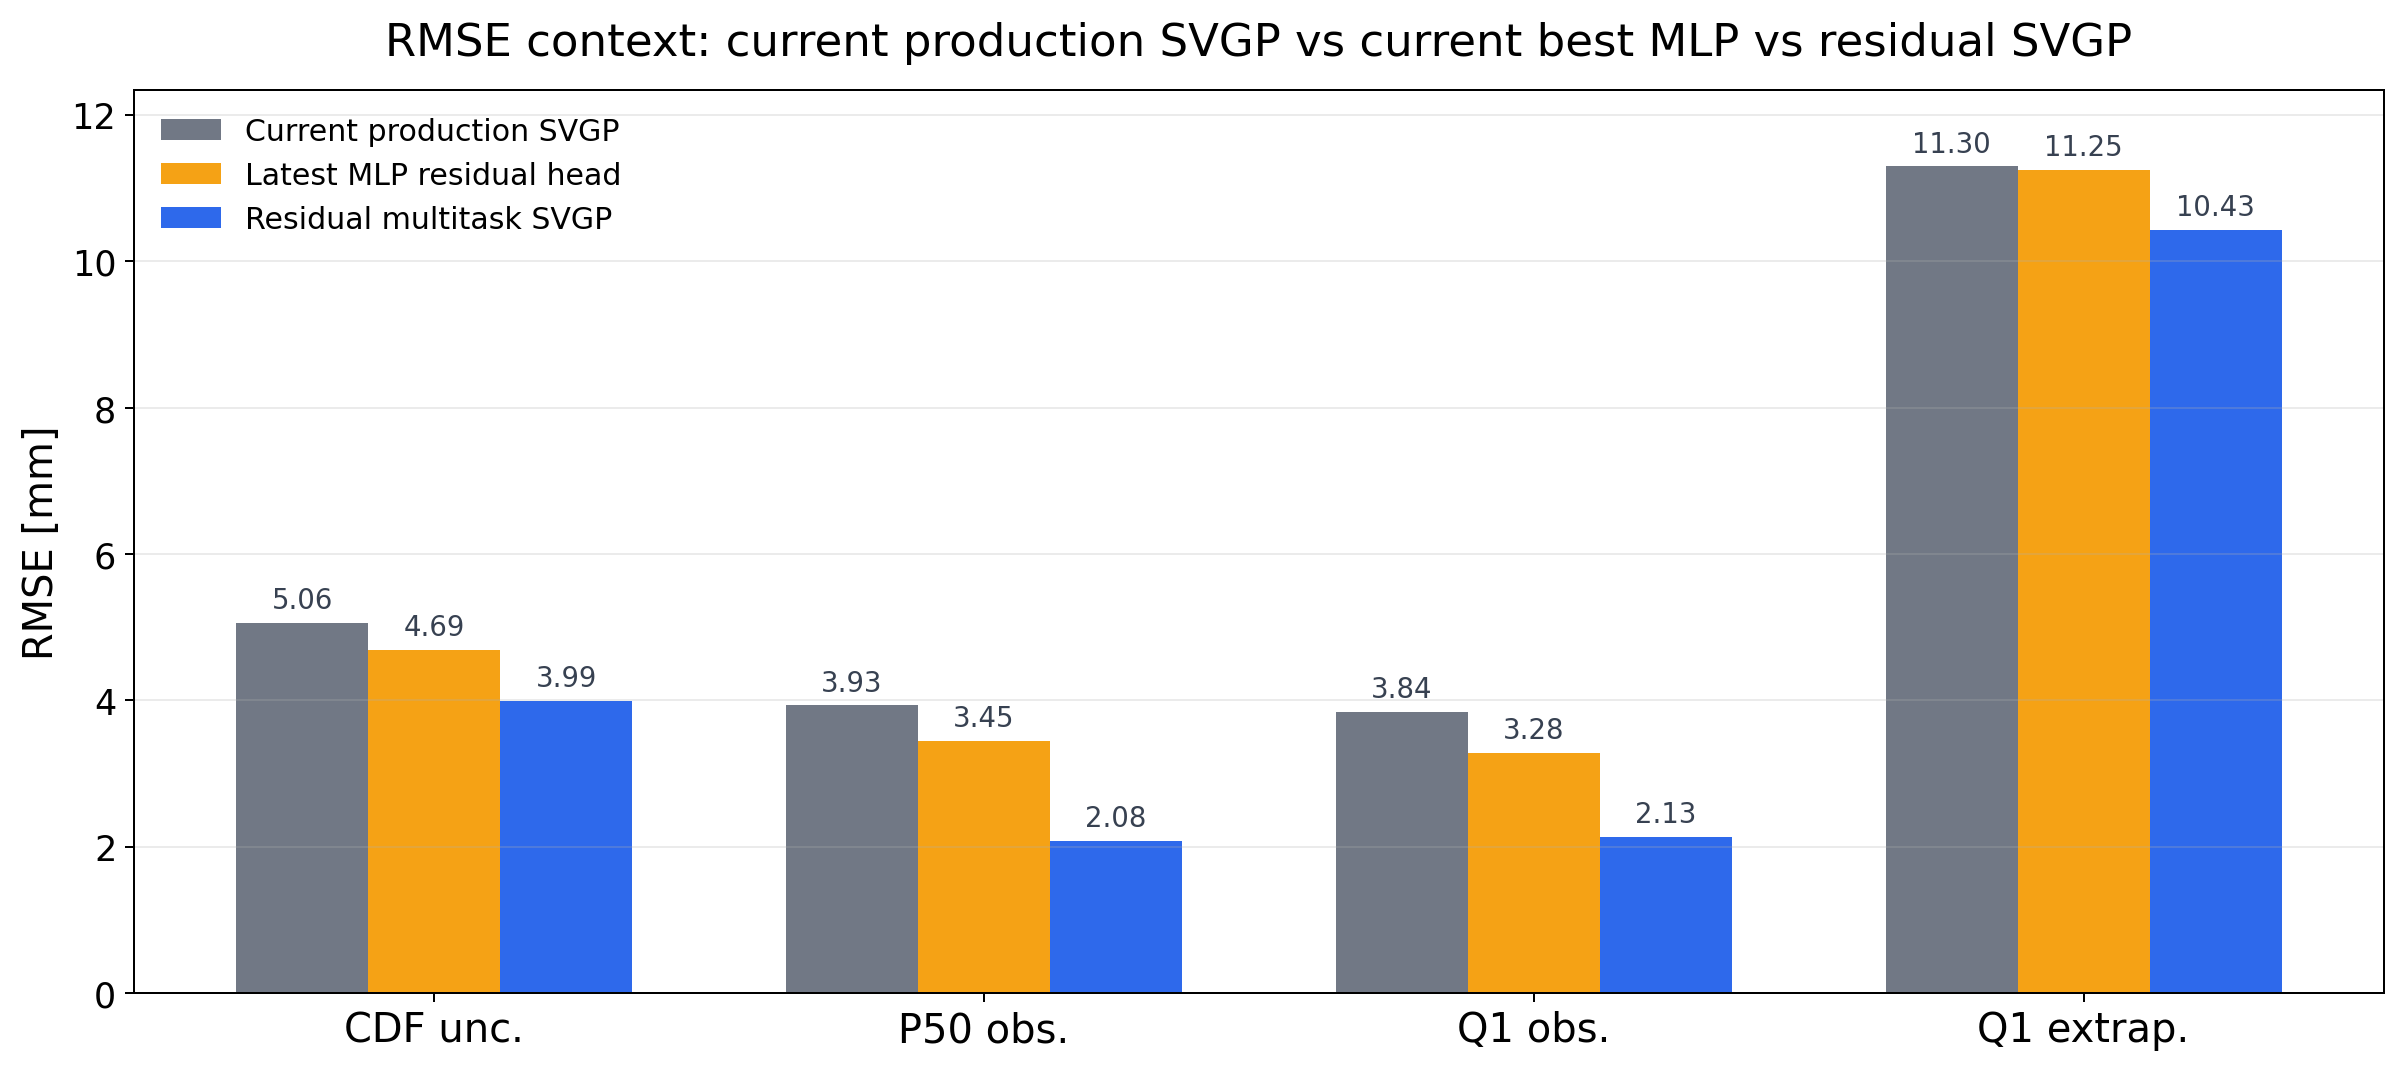
\includegraphics[width=\linewidth,height=0.52\textheight,keepaspectratio]{figs/residual_svgp_context_rmse_comparison.png}\\[0.3em]
{\scriptsize \textbf{结果} —— 残差微调相对部署模型在 CDF / P50 / Q1 上全面降低 RMSE。}
\end{columns}
\vspace{0.4em}
\begin{center}\large\good{数据证明了系统性差异，微调有用。}\end{center}
\end{frame}

% ==================================================================
\section{鲁棒性：LONO 与数据敏感性}

% ------------------------------------------------------------------
\begin{frame}{LONO：residual win 能否承受未见喷嘴？}
\small
\begin{block}{Protocol}
\begin{itemize}\setlength\itemsep{2pt}
  \item 依次 hold out Nozzle 1, 2, 4, 5, 6；\textbf{Nozzle0 留在训练集}作为第一代 anchor。
  \item 每个 fold 从 Stage-1$\to$2$\to$3 重新训练，不泄漏 production checkpoint。
  \item arms: family-head teacher, residual FH, residual-FiLM。
\end{itemize}
\end{block}
\vspace{0.1em}
\begin{center}
\scriptsize
\renewcommand{\arraystretch}{1.14}
\setlength{\tabcolsep}{4.2pt}
\begin{tabular}{@{}lrrrr@{}}
\toprule
\textbf{聚合} & \textbf{Family head} & \textbf{Residual FH} & \textbf{Residual-FiLM} & \textbf{HA / NS} \\
\midrule
全部 5 folds & 8.32 $\pm$ 2.33 & 6.95 $\pm$ 4.05 & 6.96 $\pm$ 4.08 & 11.69 / 11.10 \\
\rowcolor{winrow}
去掉 N6 的 4 folds & 7.44 $\pm$ 1.46 & \textbf{5.16 $\pm$ 0.65} & \textbf{5.15 $\pm$ 0.67} & 11.93 / 11.37 \\
\bottomrule
\end{tabular}
\end{center}
\vspace{0.25em}
\footnotesize
在 in-family folds 上，residual conversion 将 family-head RMSE 降低 \good{31\%}
（7.44$\to$5.16），同时显著降低 fold-to-fold spread。N6 作为 OOD stress fold 单独报告。
\end{frame}

% ------------------------------------------------------------------
\begin{frame}{LONO：逐 fold 读取}
\small
\begin{center}
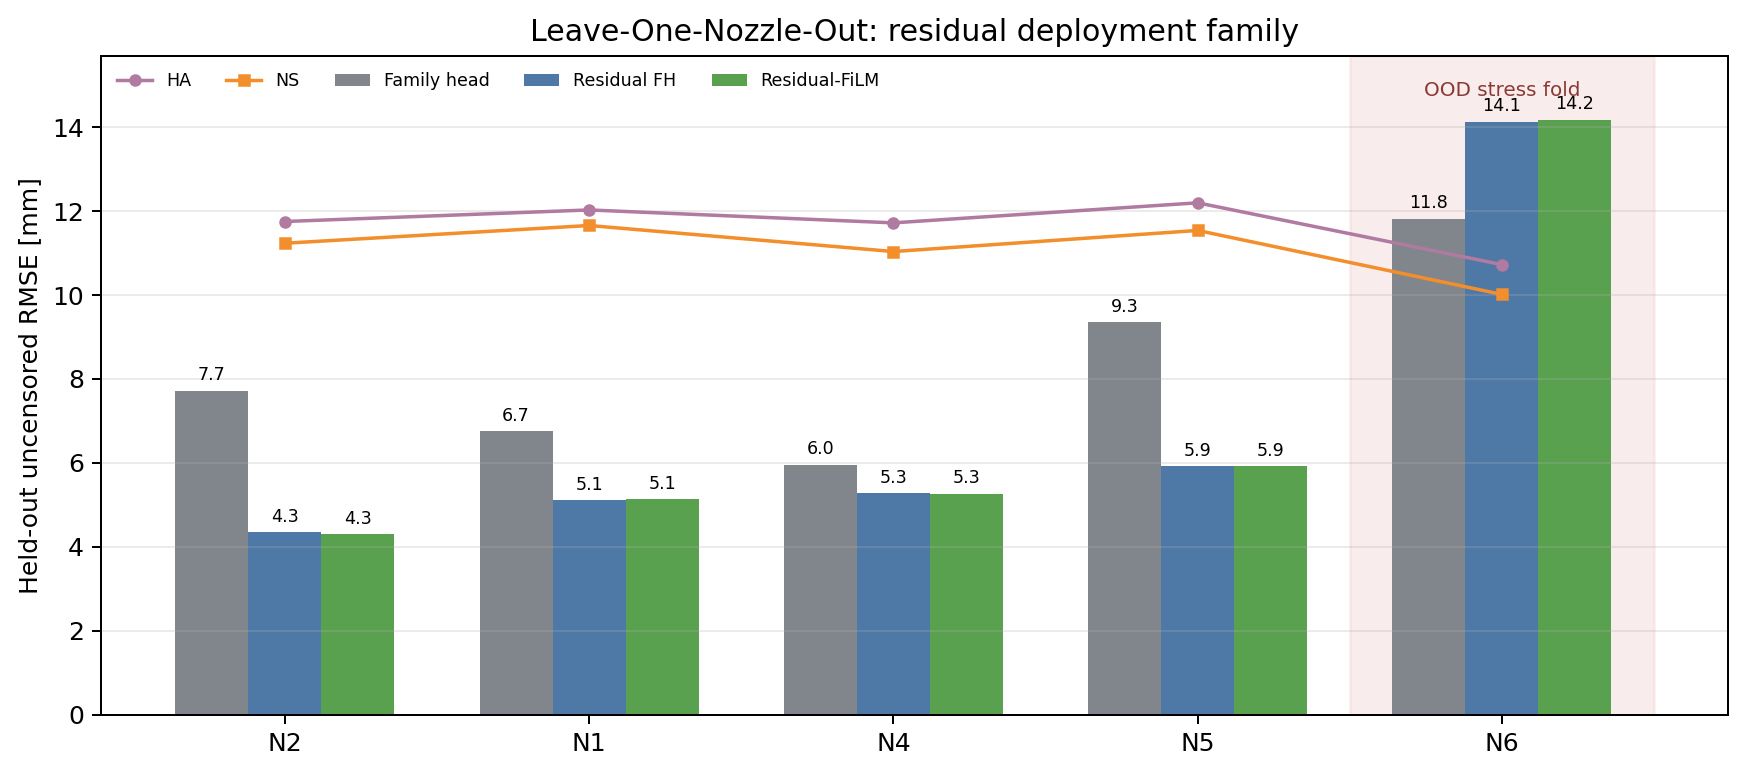
\includegraphics[width=0.92\textwidth]{figs/lono_modified_only_rmse_by_fold.png}
\end{center}
\vspace{-0.2em}
\footnotesize
\centering
Residual FH 改善所有 in-family folds：N2 \good{-3.37}、N1 \good{-1.64}、
N4 \good{-0.68}、N5 \good{-3.43} mm。N6 \warn{+2.31} mm，是明确 regression。
\end{frame}

% ------------------------------------------------------------------
\begin{frame}{LONO：结论}
\small
\begin{itemize}\setlength\itemsep{3pt}
  \item \textbf{MLP residual deployment win 可以泛化到 in-family 未见喷嘴。}
        四个 in-family held-out nozzles 上 residual arms 都超过 family-head teacher。
  \item \textbf{偏差被修复。} family head 的过预测（+3 到 +8 mm）被 residual conversion
        拉回到 4-fold mean bias \good{+0.78 mm}。
  \item \textbf{LONO 下 FH $\approx$ FiLM。} 每个 fold 相差在 0.04 mm 内；FiLM 的域内优势
        没有转化成未见喷嘴迁移优势。
  \item \textbf{N6 是真实 stress fold。} 所有 MLP arms 都掉到 12--14 mm，并且 residual arms
        严重 under-predict。这提示需要单独 OOD 研究，而不是继续堆 adapter。
\end{itemize}
\end{frame}

% ------------------------------------------------------------------
\begin{frame}{数据敏感性矩阵：显式 lv2 / lv3 root}
\small
\begin{center}
\scriptsize
\renewcommand{\arraystretch}{1.12}
\setlength{\tabcolsep}{4pt}
\begin{tabular}{@{}llrrrr@{}}
\toprule
\textbf{模型} & \textbf{训练 root} & \textbf{lv2 CDF} & \textbf{lv3 CDF} & \textbf{lv2 P50} & \textbf{lv3 P50} \\
\midrule
Family head baseline & pre-QC & 5.010 & 4.901 & 3.907 & 3.785 \\
Residual FH          & pre-QC & 4.631 & 4.519 & 3.395 & 3.264 \\
Residual-FiLM        & pre-QC & 4.510 & 4.401 & 3.166 & 3.035 \\
Residual SVGP        & pre-QC & 3.987 & 3.921 & 2.077 & 2.026 \\
\rowcolor{winrow}
Residual SVGP        & lv3 QC & \textbf{3.922} & \textbf{3.848} & \textbf{1.912} & \textbf{1.829} \\
\bottomrule
\end{tabular}
\end{center}
\vspace{0.25em}
\footnotesize
所有 row 都通过显式 \texttt{--synthetic-root} 重新评估；不使用
\texttt{MLP/synthetic\_data} junction。lv3 是 target/eval cleanup 的敏感性证据，
不能替代 lv2 的主比较。
\end{frame}

% ------------------------------------------------------------------
\begin{frame}{QC retrain：清洗效应 vs 模型增益}
\small
\begin{center}
\scriptsize
\renewcommand{\arraystretch}{1.12}
\setlength{\tabcolsep}{4pt}
\begin{tabular}{@{}lrrr@{}}
\toprule
\textbf{模型} & \textbf{Cleanup} & \textbf{QC retrain} & \textbf{Net} \\
 & \scriptsize old lv3 -- old lv2 & \scriptsize QC lv3 -- old lv3 & \scriptsize QC lv3 -- old lv2 \\
\midrule
Residual FH    & \good{-0.112} & \warn{+0.071} & -0.041 \\
Residual-FiLM  & \good{-0.108} & -0.001 & -0.109 \\
\rowcolor{winrow}
Residual SVGP  & \good{-0.067} & \good{-0.073} & \good{-0.140} \\
\bottomrule
\end{tabular}
\end{center}
\vspace{0.25em}
\footnotesize
\begin{itemize}\setlength\itemsep{2pt}
  \item \textbf{主要结构收益来自 post-training：} lv2 上 5.010$\to$4.631$\to$4.510$\to$3.987。
  \item \textbf{QC retrain 不是 MLP 普遍收益：} FH 变差，FiLM 基本持平。
  \item \textbf{明确的额外收益集中在 residual SVGP：} CDF \good{-0.073}，P50 \good{-0.197}，
        q1-observed \good{-0.170}。
\end{itemize}
\end{frame}

% ==================================================================
\section{边界：低成本 adapter 在哪里停止}

% ------------------------------------------------------------------
\begin{frame}{证据：Nozzle0 不是另一个普通 used injector}
\small
\begin{center}
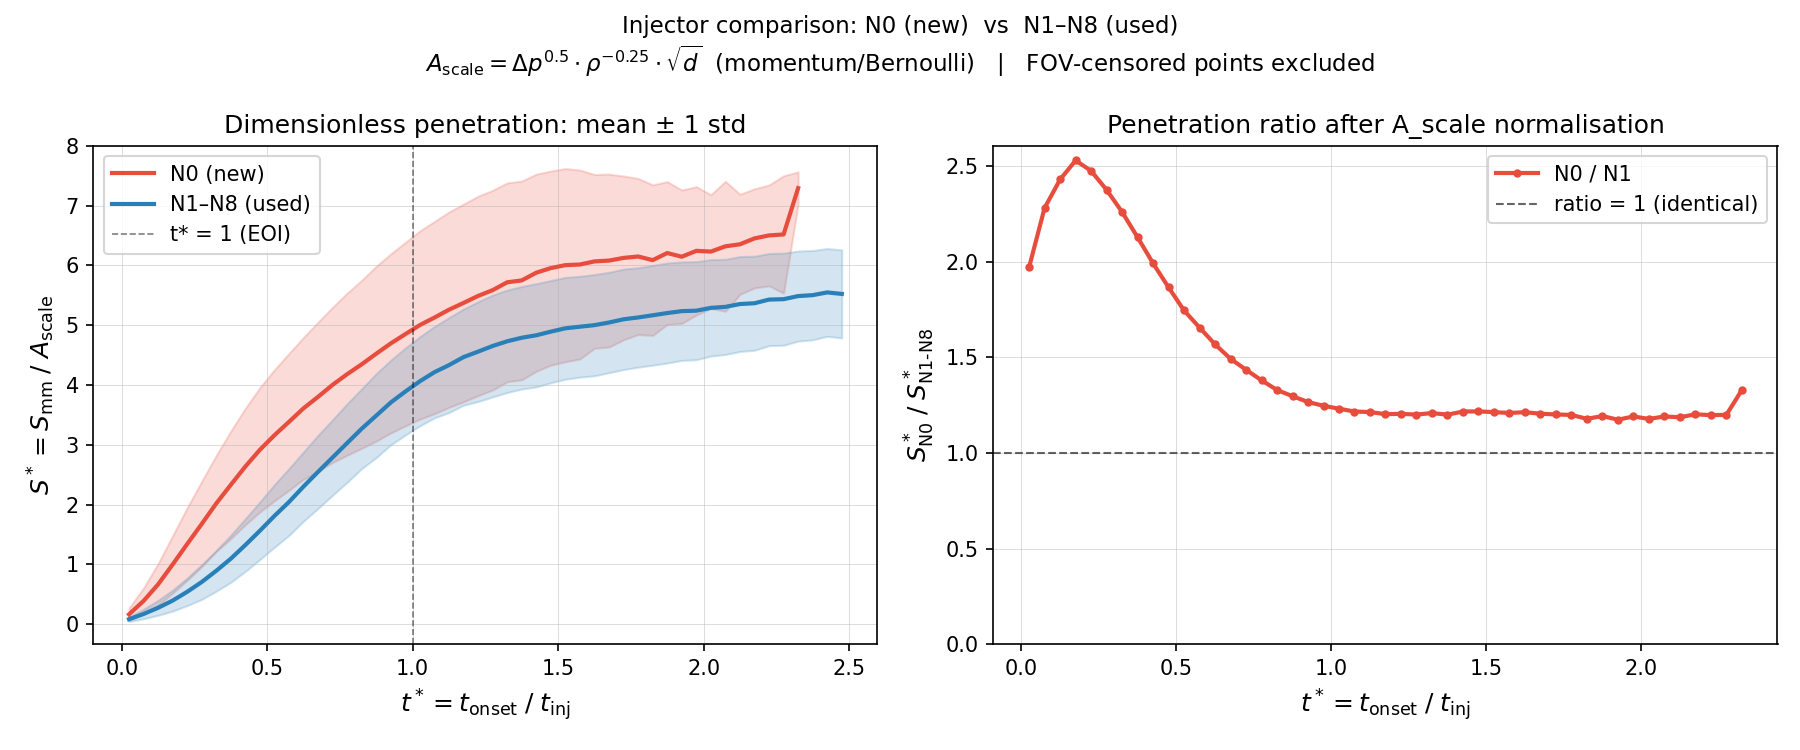
\includegraphics[height=0.58\textheight,keepaspectratio]{figs/injector_comparison_dp050.png}
\end{center}
\vspace{-0.15em}
\scriptsize
\begin{itemize}\setlength\itemsep{1pt}
  \item 即使用 momentum/Bernoulli 风格的物理缩放后，N0 的无量纲穿透曲线仍明显不同：
        early-time response 最高约为 N1--N8 的 \warn{2.5 倍}，且始终高于 1。
  \item 这说明 N0 不是“缺一个 per-family output head”，而是
        \textbf{cross-injector-distribution} 问题。
\end{itemize}
\end{frame}

% ------------------------------------------------------------------
\begin{frame}{证据：全喷嘴散点中 N0 的 early branch 分离}
\small
\begin{center}

\includegraphics[height=0.66\textheight,keepaspectratio]{figs/injector_scatter_all_nozzles.png}
\end{center}
\vspace{-0.15em}
\scriptsize
\centering
Nozzle0 在 \(t^\ast=1\) 前后占据更高的 early-time envelope，而 used injectors
大体重叠。Residual head 可以修正 family offset，但无法凭空生成冻结 trunk 未见过的表示分支。
\end{frame}

% ------------------------------------------------------------------
\begin{frame}{N6 与 N0：两种 out-of-design-family 边界}
\small
Residual head 的结构性 fallback 在新族仍属于设计族时有效；两个案例标出边界。

\vspace{0.3em}
\begin{columns}[T]
\column{0.5\textwidth}
\begin{block}{Nozzle6（LONO stress fold）}
数据最稀疏的 fold（约 20k 点）。所有 MLP arms 都掉到 12--14 mm；
residual arms 比 family head \warn{差 2.3 mm}，且强烈 under-predict。
\end{block}

\column{0.5\textwidth}
\begin{block}{Nozzle0（真正的新 injector）}
唯一第一代 injector。名义孔径相同，但实验签名不同。zero-shot 时 trunk 从未见过 N0，
RMSE 达 \warn{33.16 mm}。
\end{block}
\end{columns}

\vspace{0.4em}
\footnotesize
两者都呼应 thesis 中 Nozzle0 的跨设计族失败：per-family 输出修正不能凭空生成冻结 trunk
从未学过的表示。
\end{frame}

% ------------------------------------------------------------------
\begin{frame}{N0 few-shot adaptation：量化低成本 adapter 的上限}
\small
\begin{columns}[T]
\column{0.54\textwidth}
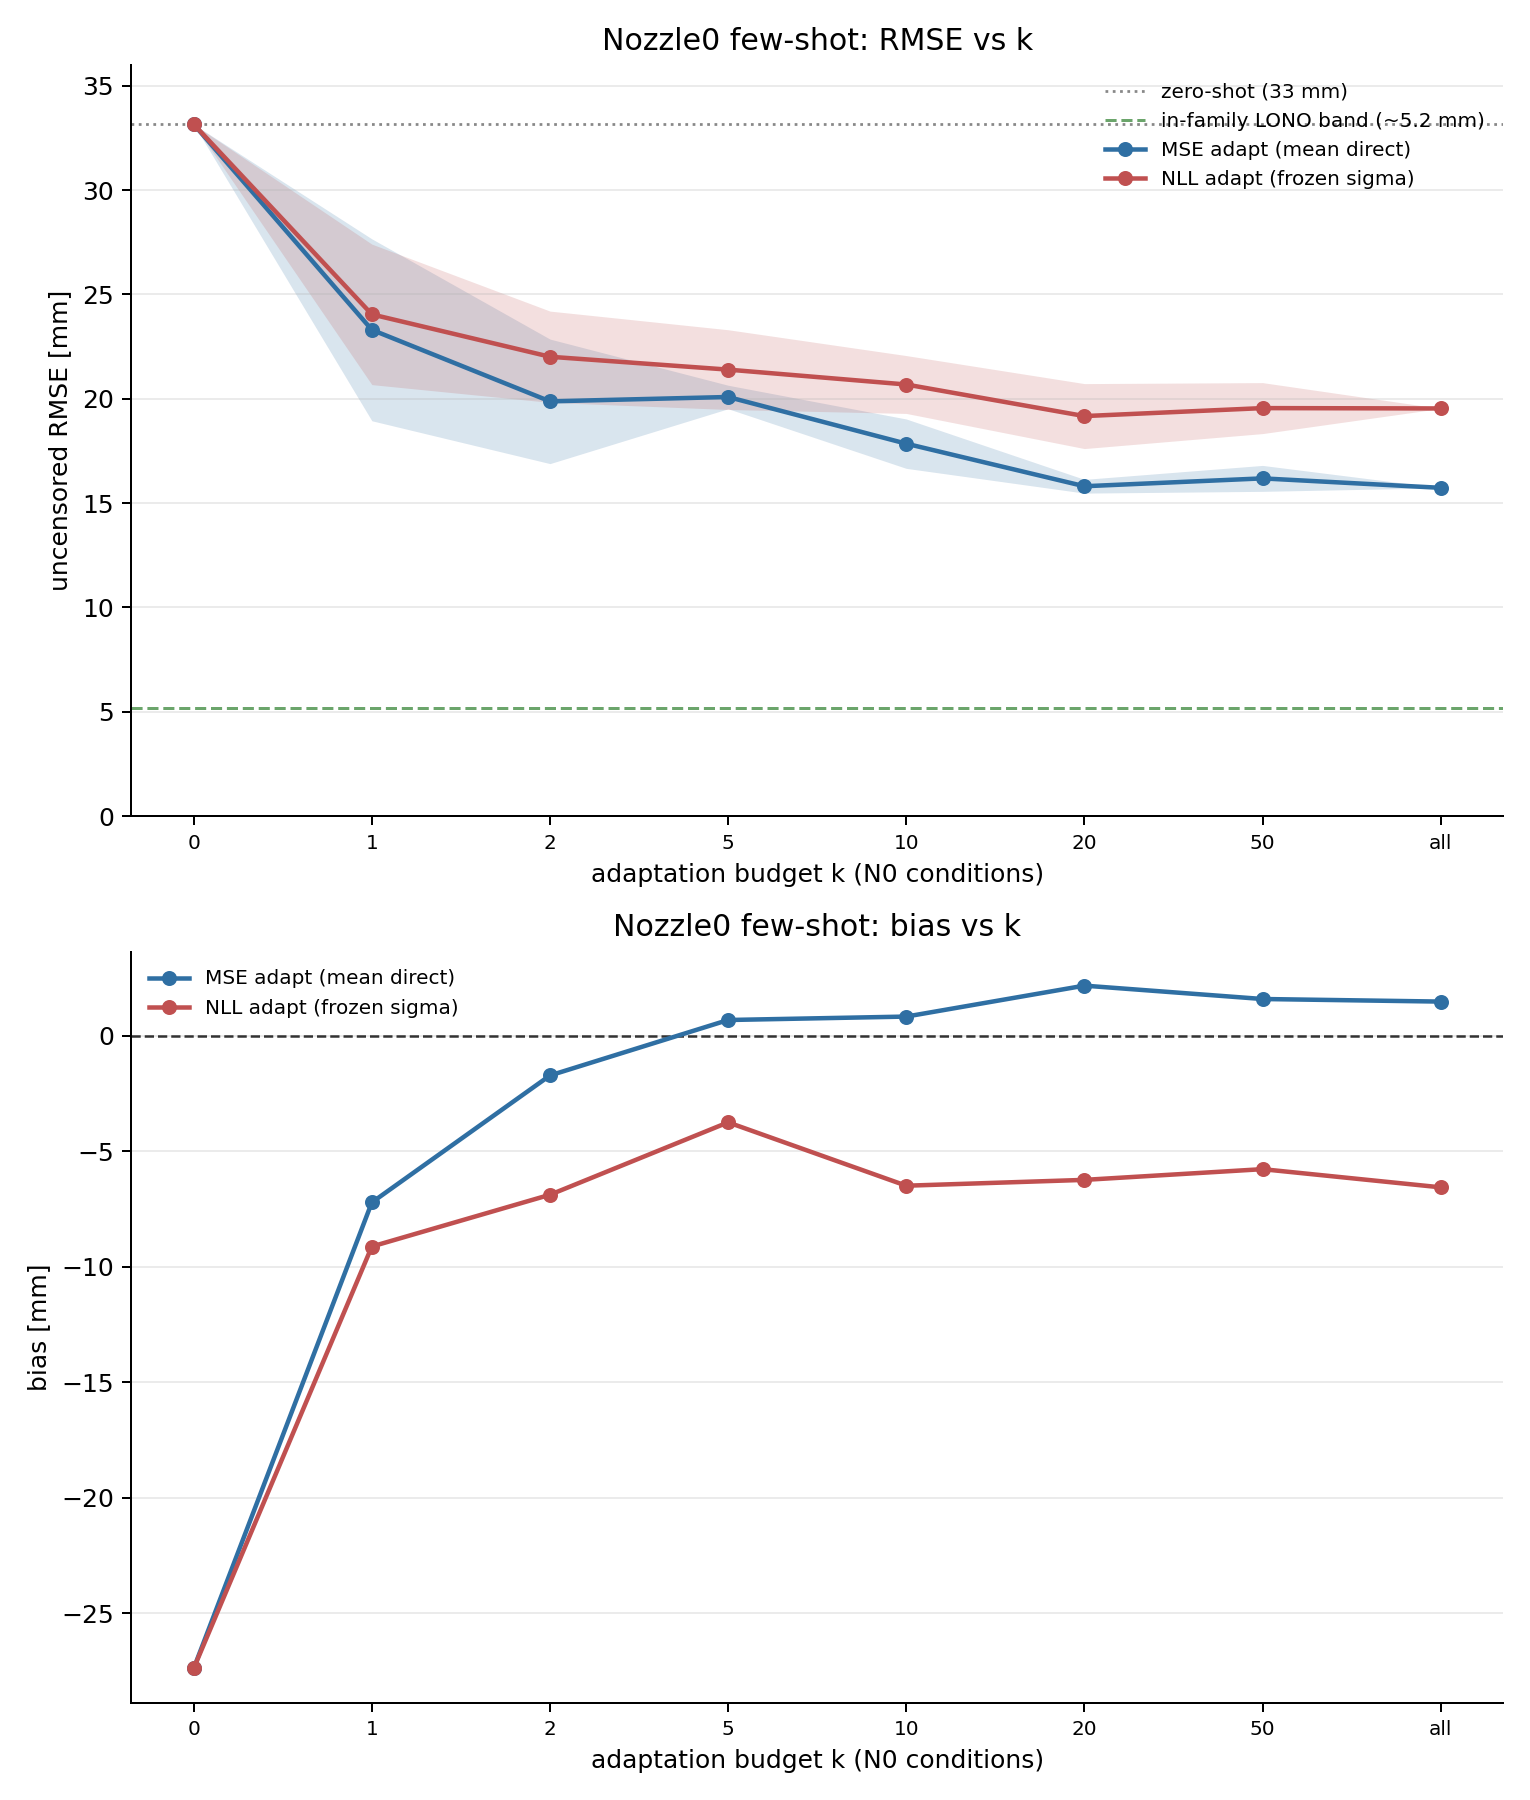
\includegraphics[width=\linewidth]{figs/n0_fewshot_adaptation_curve.png}
\column{0.46\textwidth}
\scriptsize
冻结除 \texttt{delta\_heads[0]} 外的所有参数；用 $k$ 个 N0 条件微调；
在 N0 held-out uncensored 点上评估 RMSE。
\vspace{0.3em}
\begin{tabular}{@{}rrr@{}}
\toprule
$k$ & NLL & MSE \\
\midrule
0 (zero-shot) & 33.16 & 33.16 \\
2  & 22.01 & 19.88 \\
10 & 20.68 & 17.85 \\
20 & 19.17 & 15.81 \\
all (203) & 19.54 & \textbf{15.73} \\
\bottomrule
\end{tabular}
\column{0.0\textwidth}
\end{columns}

\vspace{0.4em}
\begin{enumerate}\setlength\itemsep{2pt}
  \item \textbf{冻结 variance head 会压制 NLL adaptation。} OOD N0 上 frozen log-var 给出巨大
        $\sigma$，使 mean gradient 被下权重；MSE 直接拟合均值，floor 降低约 \good{4 mm}。
  \item \textbf{即使用 MSE，delta-only 也停在约 15.7 mm。} 它能消除全局 bias，
        但关不上 residual spread；N0 需要 trunk-level capacity。
\end{enumerate}
\end{frame}

% ==================================================================
\section{意义与总结}

% ------------------------------------------------------------------
\begin{frame}{对 thesis 结论的补充}
\small
\begin{enumerate}\setlength\itemsep{5pt}
  \item \textbf{主表出现新的最强模型。} Residual multi-task SVGP 在同一 uncensored CDF 表上达到
        \good{3.987 mm}，P50 达到 \good{2.077 mm}，超过 thesis 最强 SVGP（4.193 / 2.649）。
  \item \textbf{部署缺口被结构性闭合，但只在设计族内可靠。} 新 injector family 可以是零初始化残差，
        自动退回共享模型；预测上是否安全仍取决于是否属于设计族。
  \item \textbf{MLP branch 的 LONO 弱点被部分修复。} residual conversion 将 family head 的
        过预测修正到接近 0，并把 in-family LONO RMSE 降低 31\%。
  \item \textbf{QC-gated 结果要谨慎叙述。} lv3 是 sensitivity evidence；额外 retrain gain
        主要出现在 residual SVGP，而不是所有 MLP arms。
\end{enumerate}
\end{frame}

% ------------------------------------------------------------------
\begin{frame}{结论与下一步}
\small
\begin{block}{结论}
同一个原则——\emph{冻结热启动骨干上的加性残差}——同时推进了两个方向：
让已部署代理模型更容易扩展到新喷嘴族；并且在 SVGP 骨干上刷新主表精度与 calibration。
但这个结论只覆盖 in-design-family，可疑 OOD 族仍需要更强表示容量。
\end{block}

\vspace{0.3em}
\begin{itemize}\setlength\itemsep{2pt}
  \item 将 residual SVGP 作为候选 deployed model；QC-gated checkpoint 作为当前最强 sensitivity row。
        residual-FiLM 是最佳 MLP-only 选项，residual FH 是最简单 fallback。
  \item 保留 caveat：LONO transfer 目前只验证了 MLP arms；residual SVGP 仍需要单独 LONO fold。
  \item 对真正新 injector：不要只训练 delta head；需要同时适配 log-var head，并测试 last-block unfreeze
        或 FiLM-all-blocks。
\end{itemize}

\vspace{0.3em}
\scriptsize
\textbf{Artifacts:}
\texttt{residual\_from\_prod\_eval\_summary.csv};
\texttt{residual\_svgp\_vs\_latest\_mlp.csv};
\texttt{lono\_modified\_only/};
\texttt{cross\_dataset\_lv2\_lv3/};
\texttt{n0\_fewshot\_adaptation/}; figures under \texttt{figs/}.
\end{frame}


% ==================================================================
\appendix
\section{备份：域内训练细节}

% ------------------------------------------------------------------
\begin{frame}{附录：与代码对齐的架构细节}
\begin{center}

\includegraphics[width=0.98\textwidth,height=0.76\textheight,keepaspectratio]{figs/mlp_family_conditioning_architecture.png}
\end{center}
\end{frame}


% ------------------------------------------------------------------
\begin{frame}{训练日志怎么读}
\small
\begin{center}
\renewcommand{\arraystretch}{1.15}
\setlength{\tabcolsep}{5pt}
\begin{tabular}{@{}lrrrr@{}}
\toprule
\textbf{delta L2} & \textbf{mimic epochs} & \textbf{stop epoch} & \textbf{test loss} & \textbf{test delta RMS} \\
\midrule
0      & 10 & 104 & 2.074 & 0.816 \\
1e-4   & 10 & 44  & 2.085 & 0.818 \\
1e-3   & 10 & 110 & 2.070 & 0.813 \\
1e-2   & 10 & 84  & 2.083 & 0.810 \\
\bottomrule
\end{tabular}
\end{center}

\vspace{0.55em}
\begin{itemize}\setlength\itemsep{2pt}
  \item 四组 shrinkage 都正常 early stop。
  \item mimic 阶段先降低 production-head mismatch，再进入 raw refinement。
  \item delta RMS 聚在 0.81 左右；这个 sweep 主要调 calibration / tail，而不是改变粗尺度残差。
\end{itemize}
\end{frame}

% ------------------------------------------------------------------
\begin{frame}{Step 1：残差族头超过部署版 family head}
\small
\begin{center}
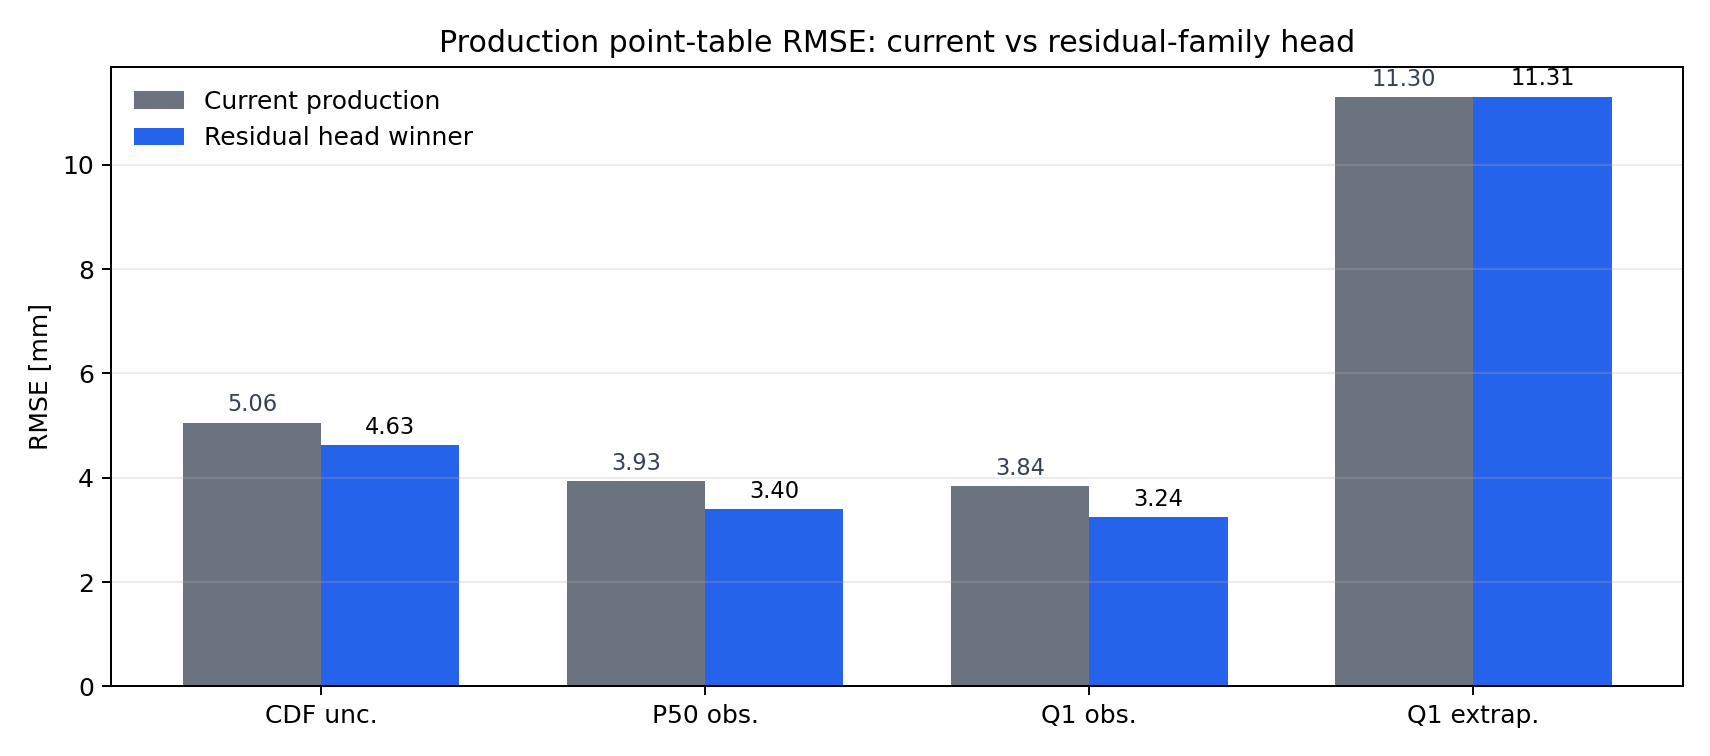
\includegraphics[width=0.56\textwidth]{figs/production_rmse_comparison.png}
\end{center}
\vspace{-0.4em}
\begin{center}
\scriptsize
\renewcommand{\arraystretch}{1.08}
\setlength{\tabcolsep}{5pt}
\begin{tabular}{@{}lrrrrr@{}}
\toprule
\textbf{模型} & \textbf{CDF RMSE} & \textbf{CDF ECE} & \textbf{CDF CRPS} & \textbf{P50 RMSE} & \textbf{Q1 obs RMSE} \\
\midrule
部署版 family head & 5.056 & 0.0708 & 2.801 & 3.931 & 3.839 \\
\rowcolor{winrow}
Residual winner (1e-4) & \textbf{4.631} & \textbf{0.0604} & \textbf{2.382} & \textbf{3.395} & \textbf{3.242} \\
\bottomrule
\end{tabular}
\end{center}
\vspace{0.2em}
\footnotesize
\centering
CDF RMSE \good{-0.425 mm}；bias 更接近 0（$+0.343\to+0.180$）；
ECE 和 CRPS 同时下降。
\end{frame}

% ------------------------------------------------------------------
\begin{frame}{Step 1：shrinkage sweep 与逐点变化}
\small
\begin{columns}[T]
\column{0.52\textwidth}
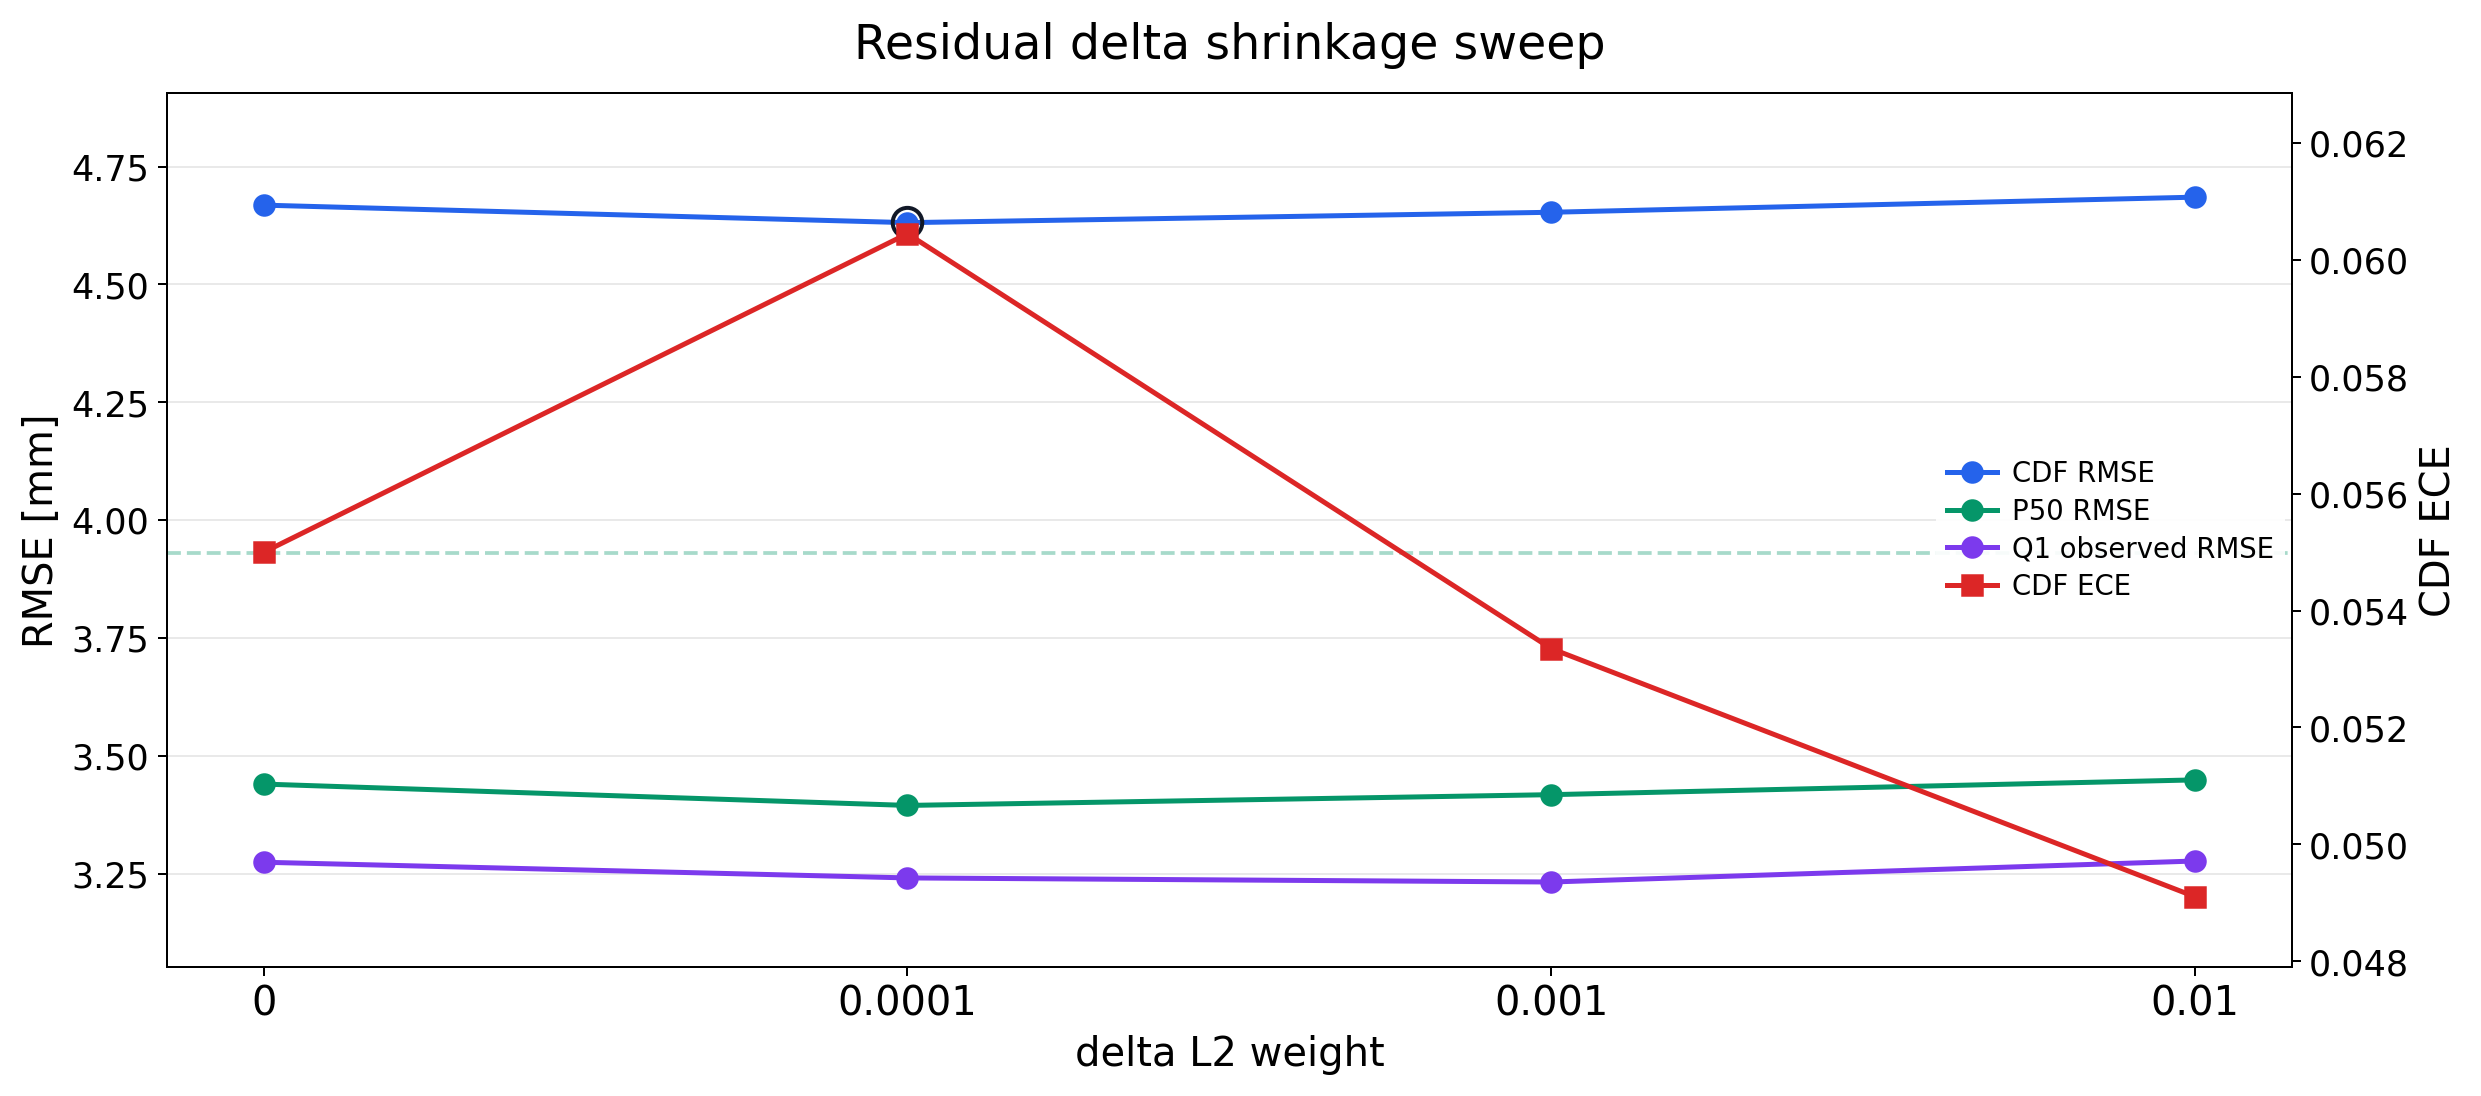
\includegraphics[width=\linewidth]{figs/delta_l2_sweep.png}
\column{0.48\textwidth}
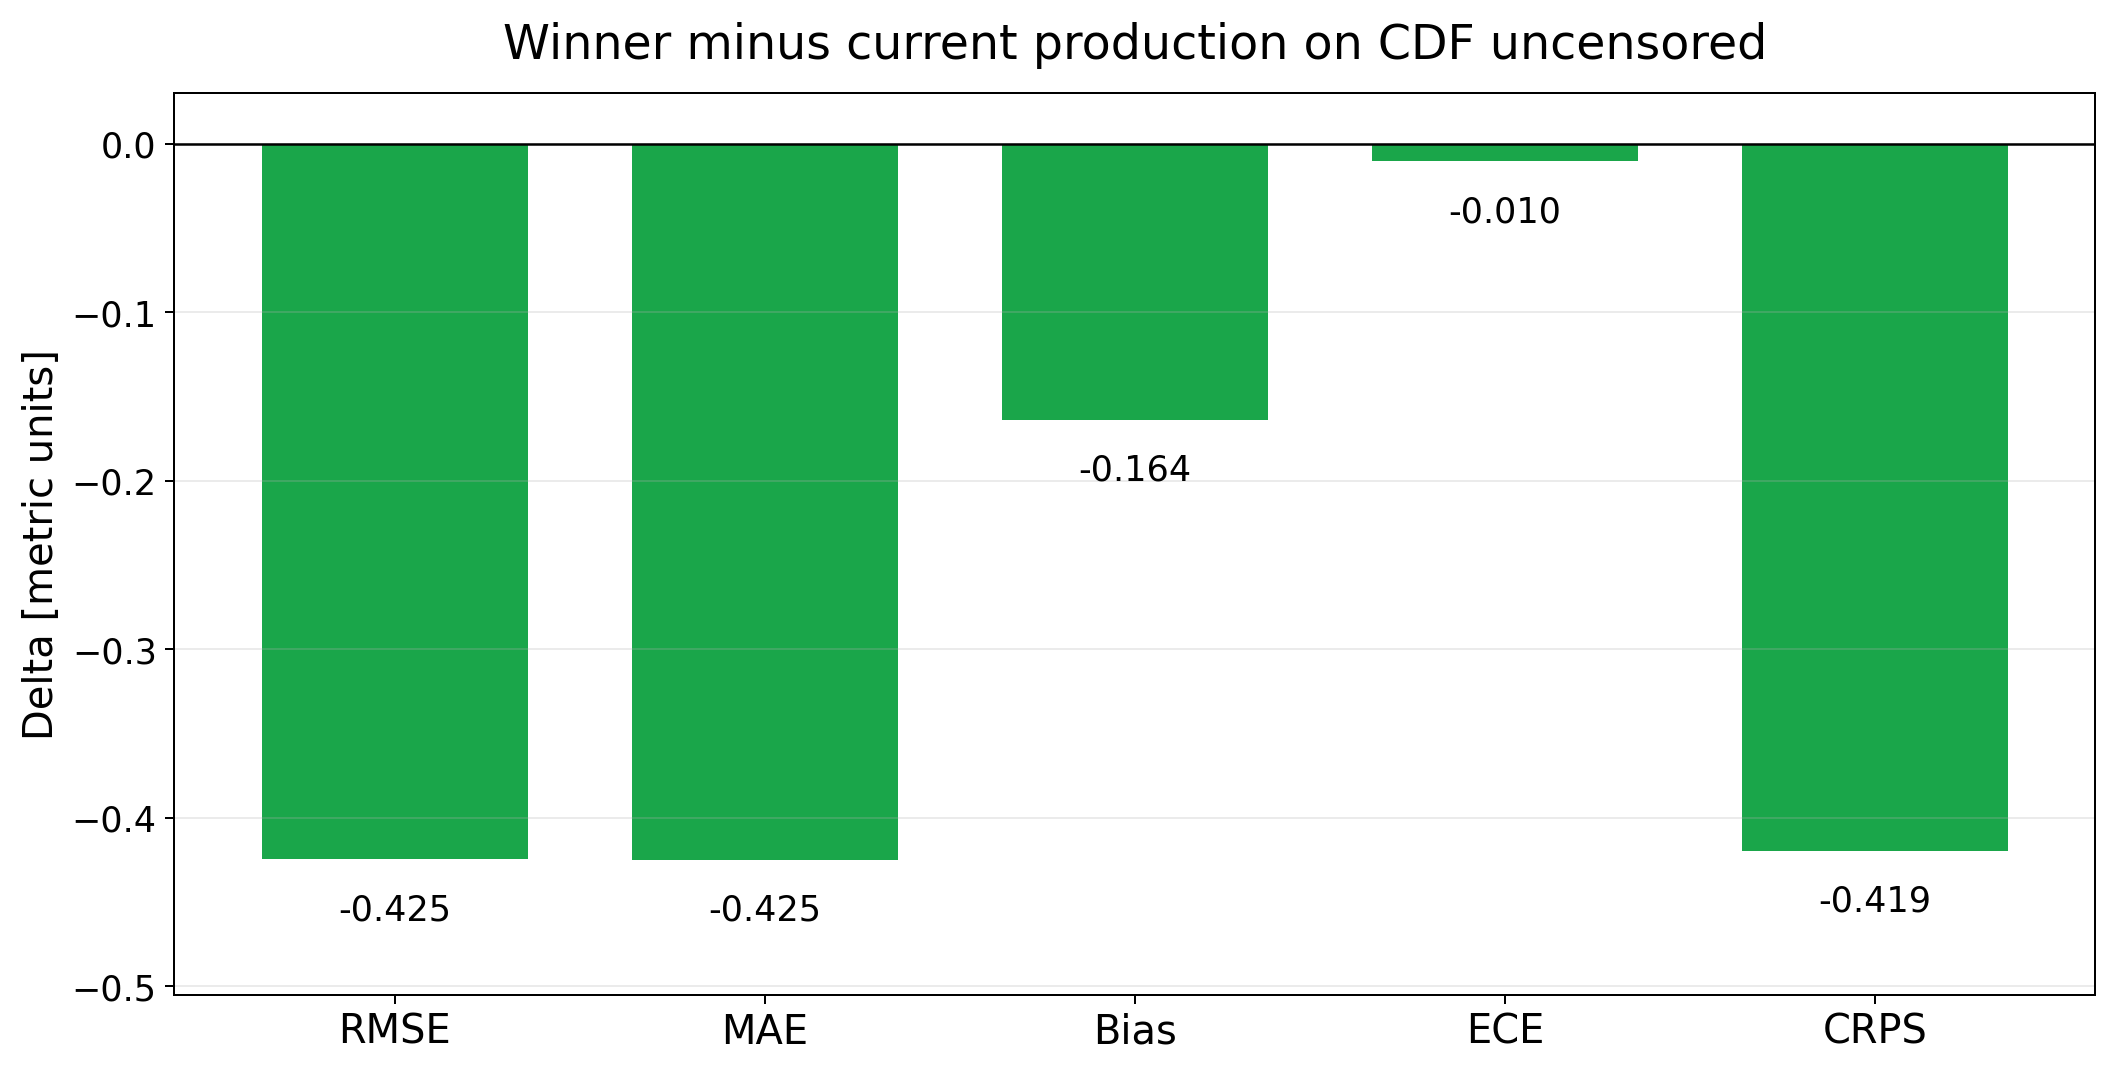
\includegraphics[width=\linewidth]{figs/winner_cdf_deltas.png}
\end{columns}
\vspace{0.3em}
\begin{itemize}\setlength\itemsep{2pt}
  \item 所有 residual settings 都超过部署版 family head；\texttt{1e-4} 给出最佳主表 RMSE。
  \item 更强 shrinkage 会改善 ECE 和 extrapolated Q1，但稍微让出主表 RMSE。
\end{itemize}
\end{frame}

% ------------------------------------------------------------------
\begin{frame}{Step 2：FiLM 表明族信息也影响表示}
\small
MLP-only 推荐 ablation：在最后一个 trunk block 后加入 identity FiLM，从 residual family head 热启动，
冻结 trunk 与 shared mean。

\vspace{0.2em}
\begin{center}
\scriptsize
\renewcommand{\arraystretch}{1.14}
\setlength{\tabcolsep}{3.4pt}
\begin{tabular}{@{}lrrrrrrr@{}}
\toprule
\textbf{模型} & \textbf{film L2} & \textbf{delta L2} & \textbf{CDF RMSE} & \textbf{CDF ECE} & \textbf{CDF CRPS} & \textbf{P50 RMSE} & \textbf{Q1 obs RMSE} \\
\midrule
Source residual FH & -- & \texttt{1e-2} & 4.685 & 0.0491 & 2.368 & 3.449 & 3.277 \\
\rowcolor{winrow}
Residual-FiLM & \texttt{1e-4} & \texttt{1e-3} & \textbf{4.510} & \textbf{0.0404} & \textbf{2.242} & \textbf{3.166} & \textbf{3.110} \\
\bottomrule
\end{tabular}
\end{center}

\vspace{0.3em}
\begin{itemize}\setlength\itemsep{2pt}
  \item CDF RMSE 再降 \good{0.176 mm}；P50 再降 \good{0.283 mm}；ECE/CRPS 同步改善。
  \item 九组 \texttt{(film,delta)} 都超过 source residual head：family signal 不只是输出偏移。
\end{itemize}
\end{frame}

% ------------------------------------------------------------------
\begin{frame}{Step 3：加性残差 multi-task SVGP 刷新主表}
\small
同一个 residual 原则搬到概率骨干：共享 SVGP 从 Stage-3 checkpoint 热启动，再加每族 residual GP。
family id 不进 kernel，只负责路由；未见族回退到共享 GP。

\vspace{0.2em}
\begin{center}
\scriptsize
\renewcommand{\arraystretch}{1.14}
\setlength{\tabcolsep}{3.4pt}
\begin{tabular}{@{}lrrrrrr@{}}
\toprule
\textbf{模型} & \textbf{delta L2} & \textbf{CDF RMSE} & \textbf{CDF ECE} & \textbf{CDF CRPS} & \textbf{P50 RMSE} & \textbf{Q1 extrap RMSE} \\
\midrule
MLP residual FH & \texttt{1e-2} & 4.685 & 0.0491 & 2.368 & 3.449 & 11.248 \\
\rowcolor{winrow}
Residual SVGP & \texttt{1e-4} & \textbf{3.987} & \textbf{0.0262} & \textbf{2.040} & \textbf{2.077} & \textbf{10.429} \\
\bottomrule
\end{tabular}
\end{center}

\vspace{0.3em}
\begin{itemize}\setlength\itemsep{2pt}
  \item 超过 single-output SVGP baseline（4.193$\to$3.987）。
  \item 相比 residual MLP，ECE 约减半（0.060$\to$0.026）。
\end{itemize}
\end{frame}

% ------------------------------------------------------------------
\begin{frame}{Step 3：Residual SVGP vs 当前最强模型}
\small
\begin{center}
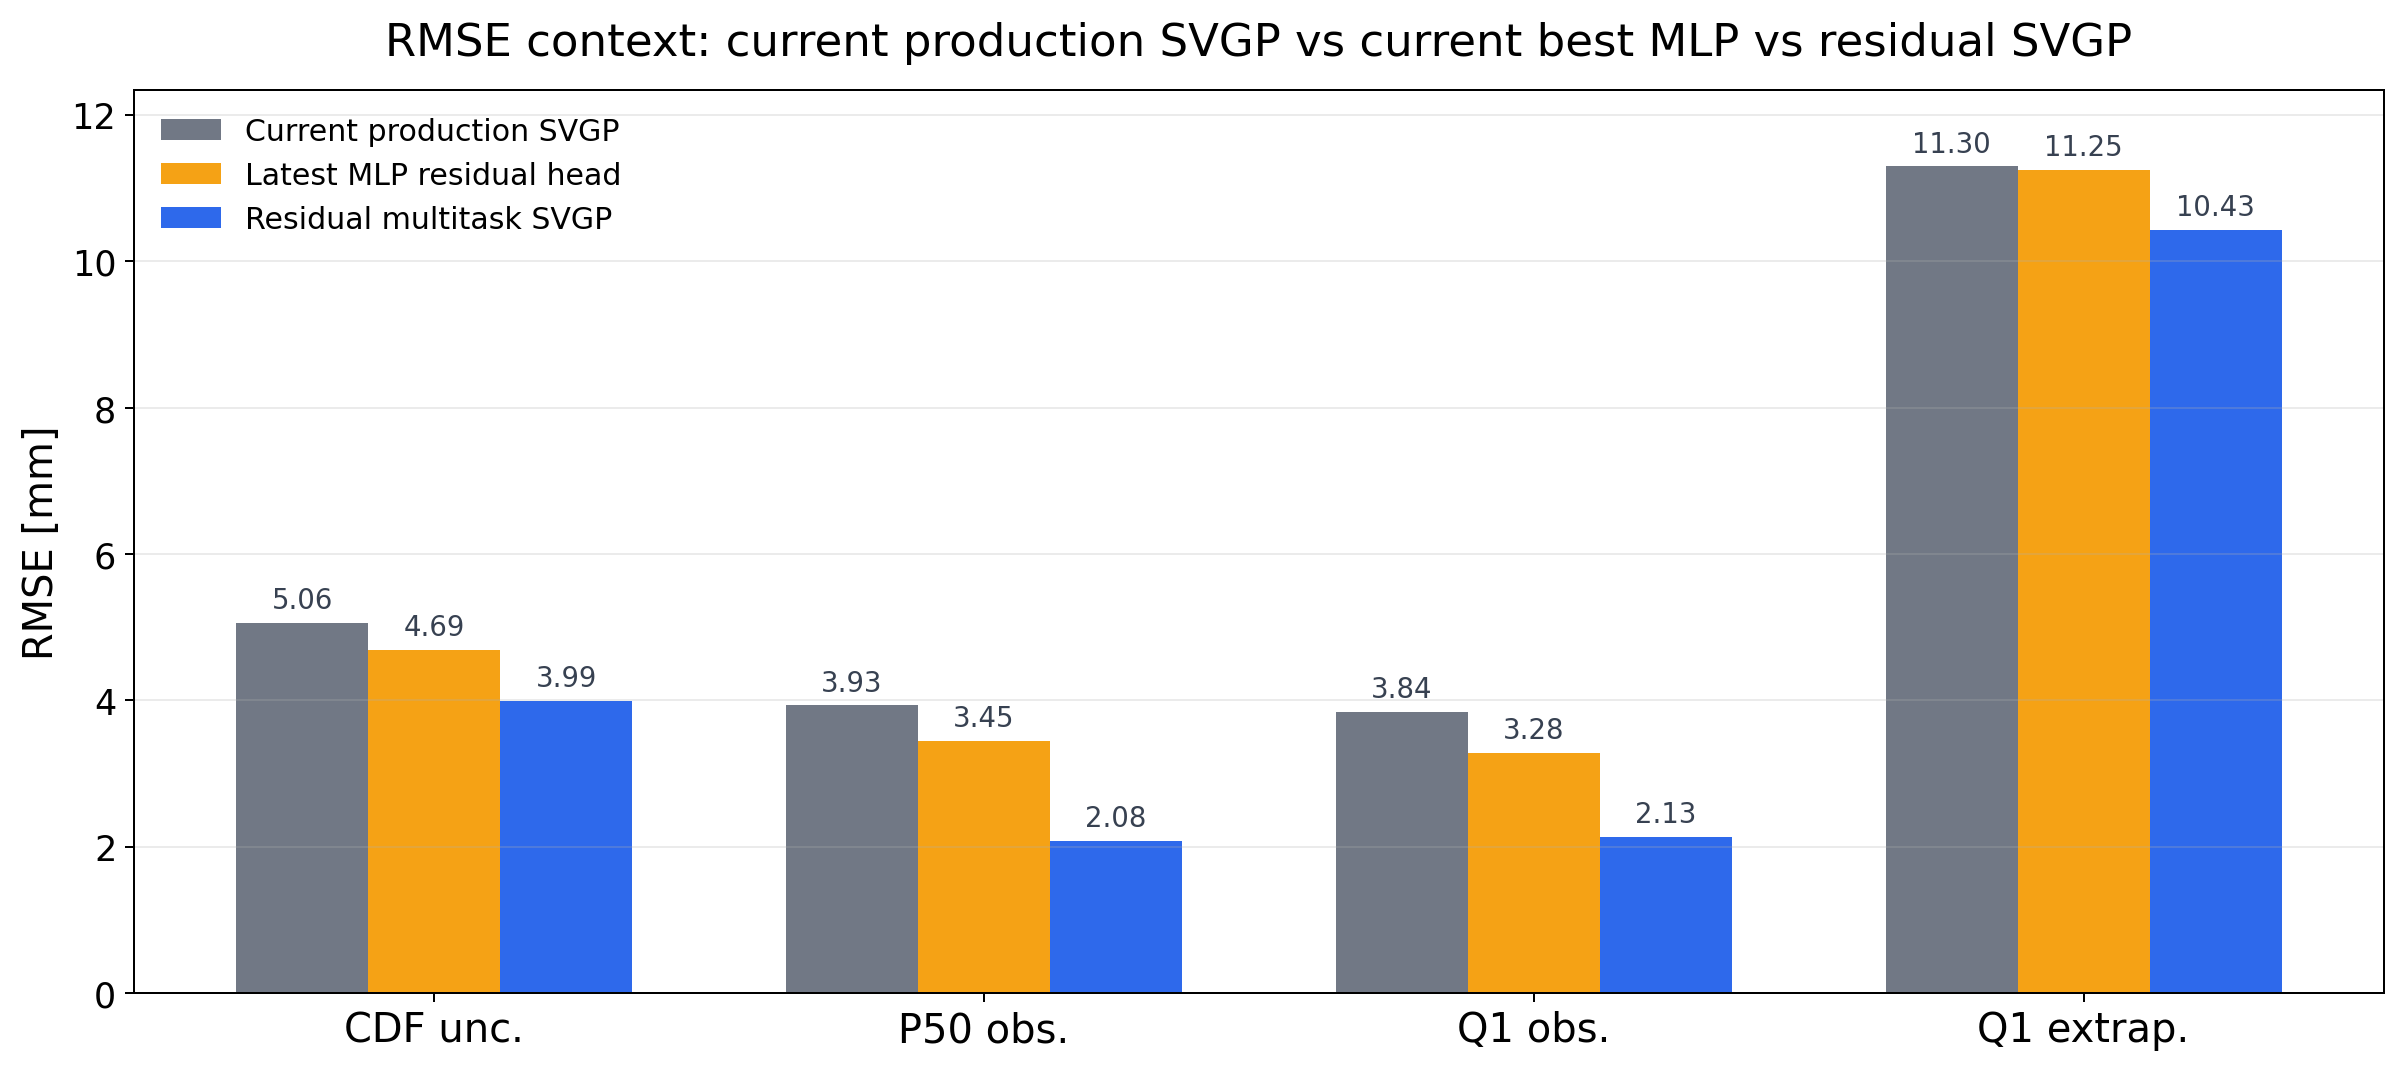
\includegraphics[width=0.90\textwidth]{figs/residual_svgp_context_rmse_comparison.png}
\end{center}
\end{frame}

% ------------------------------------------------------------------
\begin{frame}{同一主表上的爬升（lv2 uncensored CDF，542k 点）}
\small
\begin{center}
\renewcommand{\arraystretch}{1.18}
\setlength{\tabcolsep}{5pt}
\begin{tabular}{@{}lrrl@{}}
\toprule
\textbf{模型} & \textbf{CDF RMSE} & \textbf{P50 RMSE} & \textbf{来源} \\
\midrule
Naber--Siebers 物理基线 & 9.286 & -- & thesis \\
三阶段 MLP 选定模型 & 4.265 & 2.848 & thesis \\
Stage-3 SVGP & 4.193 & 2.649 & thesis 旧最强 \\
\midrule
部署版 family head & 5.010 & 3.907 & deployment variant \\
Residual FH (1e-4) & 4.631 & 3.395 & this work \\
Residual-FiLM & 4.510 & 3.166 & this work \\
\rowcolor{winrow}
Residual SVGP (1e-4) & \textbf{3.987} & \textbf{2.077} & this work 新最强 \\
Residual SVGP, QC retrain & 3.922 & 1.912 & sensitivity re-score \\
\bottomrule
\end{tabular}
\end{center}
\vspace{0.25em}
\footnotesize
MLP residual 修复了部署版 family head 的精度损失，但没有超过更简单的 single-head surrogate。
真正推进精度边界的是 residual SVGP。QC retrain 在同一 lv2 root 上还能改善 residual SVGP，
但作为 sensitivity evidence 解读。
\end{frame}

\end{document}
